\documentclass[letterpaper,journal]{IEEEtran}
\usepackage{amsmath,amsfonts,amssymb}
\usepackage{array}
\usepackage[caption=false,font=normalsize,labelfont=sf,textfont=sf]{subfig}
\usepackage{textcomp}
\usepackage{stfloats}
\usepackage{url}
\usepackage{graphicx}
\usepackage{cite}
\usepackage{booktabs}
\usepackage{tcolorbox}
\usepackage{diagbox}  % 引入斜线宏包
\usepackage[hidelinks]{hyperref}


\hyphenation{op-tical net-works semi-conduc-tor IEEE-Xplore}
% updated with editorial comments 8/9/2021

\begin{document}

\title{Understanding the Structure and Evolution of Bug Maintenance in LLM Inference Engines}

\author{\IEEEauthorblockN{Jiachen Liu\IEEEauthorrefmark{3}\textsuperscript{*}, Chaoning Zeng\IEEEauthorrefmark{3}\textsuperscript{*}, Chijin Zhou\IEEEauthorrefmark{3},
Quan Zhang\IEEEauthorrefmark{3},
Yu Jiang\IEEEauthorrefmark{4}, Geguang Pu\IEEEauthorrefmark{3} \\
\IEEEauthorblockA{\IEEEauthorrefmark{3}School of Software Engineering, East China Normal University, Shanghai, China \\
\IEEEauthorrefmark{4}School of Software, Tsinghua University, Beijing, China \\
% \\
}
}
\thanks{\textsuperscript{*}Jiachen Liu and Chaoning Zeng contributed equally to this work.}

}
% The paper headers
% \markboth{Journal of \LaTeX\ Class Files,~Vol.~14, No.~8, August~2021}%
% {Shell \MakeLowercase{\textit{et al.}}: A Sample Article Using IEEEtran.cls for IEEE Journals}

% \IEEEpubid{0000--0000/00\$00.00~\copyright~2021 IEEE}
% Remember, if you use this you must call \IEEEpubidadjcol in the second
% column for its text to clear the IEEEpubid mark.

\maketitle

\begin{abstract}
Large language model (LLM) inference engines are complex systems whose reliability affects correctness and service availability. This paper presents a code-centered empirical study of how bugs manifest, where faults reside, how developers repair them, and how repair scope evolves in six widely used open-source engines. We identify 50,121 pull requests related to bug fixing, submitted from the start of each project to March 2026. Among these, 12,707 were merged into their respective project codebases and manually verified as actual bug fixes, forming our study corpus. For each verified fix, we connect its observed symptom to the faulty code, repair operation, and patch scope. We find that 31.5\% of the verified fixes address bugs that directly affect correctness or availability. Symptom distributions also differ substantially across architectural layers. Maintenance is concentrated in both location and activity: the top 20\% of files account for 79.6\% of bug-fixing occurrences, while logic correction and adaptation make up 73.6\% of repair operations. From 2023 to early 2026, fixes increasingly span multiple files, while Hardware Adaptation occupies a growing share of bug-fixing activity. Together, these findings provide an empirical basis for improving how bugs are detected, localized, and repaired in LLM inference engines.
\end{abstract}
\begin{IEEEkeywords}
LLM inference engines, empirical study, software maintenance, software evolution.
\end{IEEEkeywords}

\section{Introduction}
The reliability of a large language model (LLM) service depends not only on the model, but also on the inference engine beneath it. Every request passes through a long execution path that covers model preparation, runtime orchestration, and hardware execution. Modern engines make this path faster through advanced scheduling, memory management, heterogeneous execution, and distributed serving~\cite{yu2022orca,kwon2023pagedattention,aminabadi2022deepspeed,zheng2024sglang,zhong2024distserve,park2026inferenceengines}. They must also support a growing range of models, optimization methods, and deployment environments. As a result, an inference engine is no longer a simple model runtime. It is a large systems stack whose layers must evolve together while preserving correctness, availability, and performance across environments.

This combination of optimization and broad compatibility makes inference-engine bugs both harmful and difficult to maintain. A faulty engine may silently corrupt an output, disrupt a service through a runtime or resource failure, or break only in a specific deployment environment. These failures are also difficult to diagnose. An incorrect output can easily be mistaken for a weakness of the model, while a latency increase may be blamed on the workload or hardware. Even after a failure is confirmed as an engine bug, its visible symptom may be far from its source. The fault may reside in the computation layer, the runtime control plane, or a deployment interface. Its repair may require either a one-line correction or a coordinated change across several modules. A symptom taxonomy can describe how an engine fails, but reliability is improved through decisions about code: where to test, where to search for a fault, and how broadly to validate a fix. Making these decisions requires connecting observed failures to the code regions that cause them and to the changes needed to repair them. Such connections turn bug observations into actionable guidance for testing and maintenance.

Prior work has studied bugs in deep learning applications, frameworks, and compilers, producing taxonomies of symptoms, causes, and affected components~\cite{islam2019bugs,humbatova2020taxonomy,yang2022frameworkbugs,chen2023frameworkbugs,shen2021compilerbugs,du2021compilerbugs}. General software-engineering studies have also shown that fixes follow recurring patterns and that faults often concentrate in a small part of a codebase~\cite{pan2009bugfixpatterns,sobreira2018dissection,liu2020vulnerabilitydistribution}. Most closely related, Liu et al.~\cite{liu2026firstlook} studied 929 bugs from five LLM inference engines and characterized their failure types, repair behavior, and evolution. These studies explain \emph{what kinds of bugs occur}. However, they leave a broader maintenance question open: \emph{how is bug maintenance structured inside the codebase, and how does it evolve over time?}

Answering this question is challenging for three reasons. First, the relation between symptoms and faulty code is many-to-many. The same symptom may originate in different layers, while one layer may produce very different failures. Issue categories alone therefore cannot identify where developers should inspect or test. Second, patch size does not reveal repair intent. Similar-sized patches may perform different operations, and one fix may combine several operations across code entities. Measuring changed lines alone therefore misses both the meaning and the spread of maintenance work. Third, inference engines evolve rapidly and at different rates. Changes in project size or bug mix can obscure whether repairs themselves are reaching a wider code surface or shifting their architectural focus. Addressing these challenges requires a joint analysis of failure symptoms, code locations, and repair patches across projects and over time.

In this paper, we take a code-centered view of maintenance in LLM inference engines. We connect each observed failure to two forms of code evidence: where the fault resides and how developers repair it. The first captures the affected architectural layer and code entities. The second captures the repair operation and repair scope, including patch breadth and architectural distribution. Rather than report these dimensions in isolation, we follow each bug from its external effect to its internal location and then to the resulting code change. By studying these connections across projects and over time, we reveal where maintenance effort accumulates, what developers repeatedly change, and how repair boundaries evolve.

We use this view to answer three research questions:
\begin{itemize}
    \item \textbf{RQ1---Failure localization:} Across LLM inference engines, how are observed failure symptoms associated with the architectural layers in which faults reside?
    \item \textbf{RQ2---Repair structure:} How is bug-fixing work structured across code entities and architectural layers?
    \item \textbf{RQ3---Repair evolution:} How does the scope of bug fixes evolve over time?
\end{itemize}

To answer these questions, we conduct the largest code-centered empirical study of LLM inference-engine bugs to date. We study six widely used open-source engines: llama.cpp, vLLM, DeepSpeed, MLC-LLM, TensorRT-LLM, and Text Generation Inference (TGI). Together, they cover cloud and local deployment, single and multi-device execution, and a wide range of hardware and software backends. We collect all 50,121 bug-fix-related pull requests submitted to their official repositories from the start of each project to March 2026. We then select the pull requests merged into the projects' codebases and manually review each one to determine whether it implements a bug fix. This process yields a study corpus of 12,707 merged and manually verified bug-fixing pull requests. For each fix, we combine repository metadata, development discussions, and the complete code patch. We classify failures into ten symptom types, locate faulty code in nine architectural layers, and identify nine types of repair operations. We then map the fixes to code entities, measure repair scope through patch breadth and architectural distribution, and track its monthly evolution. This process gives us an end-to-end view of each repair, from the failure observed by a user to the code modified by a developer.

Our study reveals three main properties of inference-engine maintenance. First, failures are strongly shaped by system architecture. Bugs that directly threaten correctness or availability, i.e., incorrect outputs, runtime crashes, and model-loading failures, account for 4,001 of the 12,707 studied fixes (31.5\%). Some layers have narrow and recognizable failure signatures. Bugs in build and release tooling mainly prevent compilation or installation, while bugs in user-facing configuration and entry points often appear as API or argument-parsing errors. By contrast, bugs in request scheduling and runtime control can affect correctness, availability, or resource use. Symptoms can therefore provide strong localization clues for specialized layers, whereas failures in the central execution logic require broader diagnosis and testing.

Second, maintenance risk is highly concentrated. The top 20\% of files account for 79.6\% of bug-fixing occurrences, and the top 20\% of functions account for 68.4\%. The pattern appears in all six engines. Hotspot files therefore contain multiple functions that repeatedly participate in bug fixes, rather than only one isolated faulty function. Repair work is concentrated as well: Logic Correction and Adaptation account for 14,702 of 19,965 repair-operation instances (73.6\%). Together, these results show that the main maintenance burden comes from a limited code surface and the continuing need to preserve correct behavior across evolving hardware and software.

Third, bug fixes are becoming less local. Most fixes are still compact. The median patch changes only 14 lines, but large repairs are not rare: roughly 10\% changes at least 165 lines. More importantly, from 2023 to early 2026, repairs increasingly spanned several files instead of remaining within one, while Hardware Adaptation occupied a growing share of bug-fixing activity. This shift means that inference-engine maintenance is moving from isolated edits toward coordinated changes across related parts of the codebase and a more prominent hardware-adaptation focus. Review and regression testing must therefore follow the full change, because checking only the first failing file can overlook related changes.

These findings change the view of inference-engine reliability in several ways. Bugs are not spread evenly across a repository; they form stable code hotspots. Symptoms are not independent of architecture; they carry different amounts of information about fault location. Repairs are not dominated by generic cleanup; they mainly correct logic and adapt behavior across environments. Finally, maintenance does not remain equally local as engines mature; the code boundary of a fix tends to widen and its architectural focus can shift. This knowledge can guide hotspot-based testing, architecture-aware debugging, and code-aware automation for LLM systems.

In summary, this paper makes the following contributions:
\begin{itemize}
    \item We present the largest code-centered empirical study of LLM inference-engine bugs, covering 12,707 merged and manually verified bug-fixing pull requests from six open-source engines. We connect failure symptoms, faulty code, and repair patches in an analysis framework.
    \item We characterize bug-fixing work in LLM inference engines. We show how system architecture shapes failure symptoms, where maintenance effort concentrates, and how repair operations differ across architectural layers.
    \item We provide a large-scale view of how inference-engine repair scope changes over time, including patch breadth and architectural distribution. Our results expose an expanding repair boundary and growing Hardware Adaptation focus, guiding testing, review, and automated repair for LLM serving systems.
\end{itemize}

\begin{tcolorbox}[
    colback=white,
    colframe=black,
    boxrule=0.5pt,
    arc=1pt,
    left=4pt,
    right=4pt,
    top=3pt,
    bottom=3pt,
    before skip=4pt,
    after skip=0pt
]
\textbf{Artifact:} Code and data are available at \url{https://github.com/Ellliot-ECNU/llm-engine-bugs}.
\end{tcolorbox}

\section{Background}

\subsection{LLM Inference Service Architecture}

A typical LLM service separates application orchestration from model execution, as shown in Fig.~\ref{fig:inference_engine}. Upper-layer applications construct prompts, retrieve context, or invoke external tools and data sources; the orchestration layer packages this information into a generation request and consumes the returned tokens. The \emph{inference engine} is the serving and runtime stack that processes the request on one or more compute devices. It does not include model training or application-side logic such as retrieval-augmented generation.

\begin{figure}[t]
    \centering
    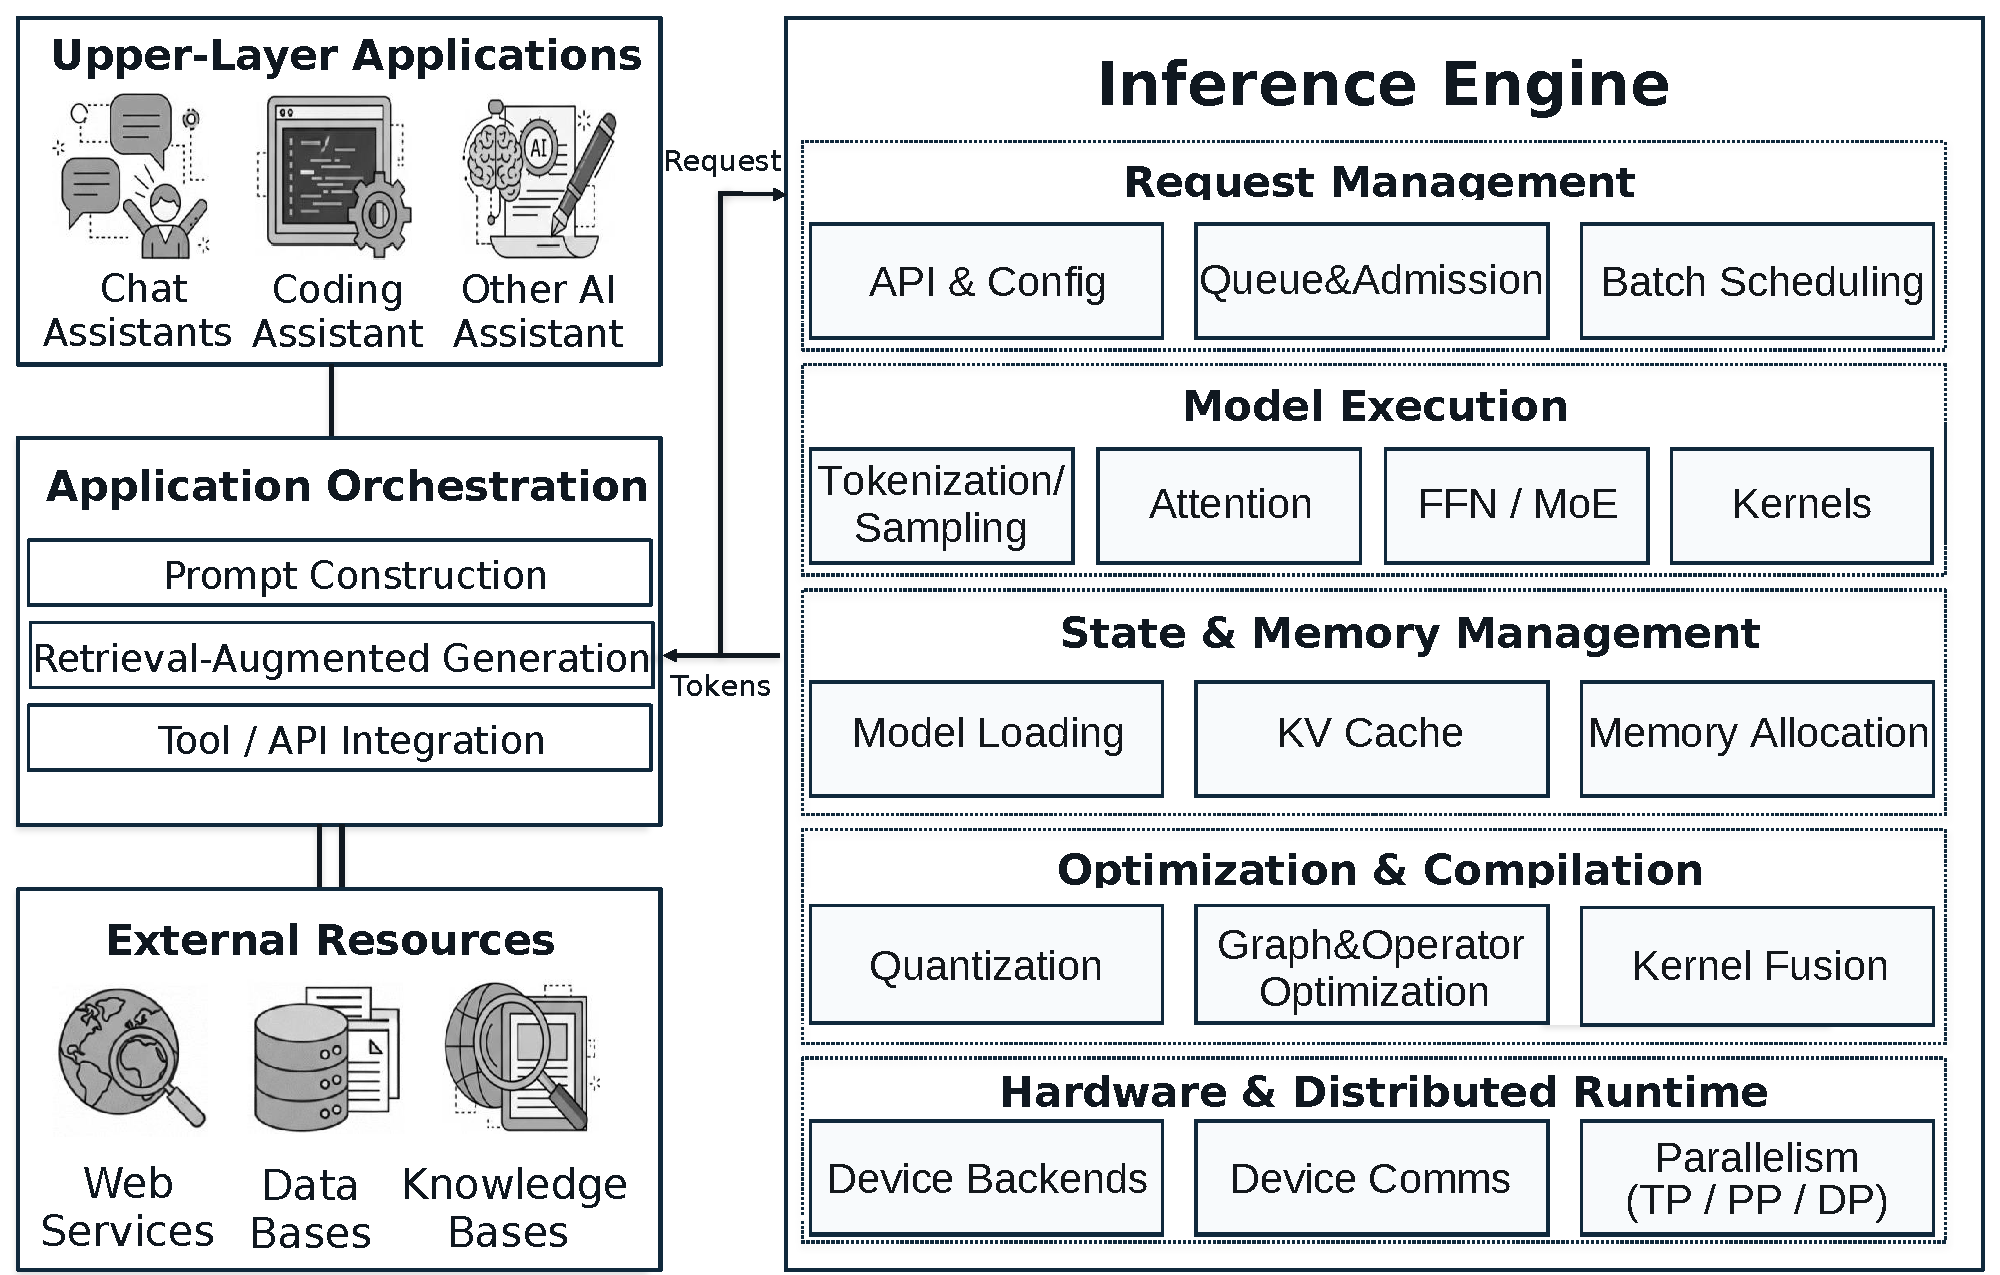
\includegraphics[width=0.95\linewidth]{fig/inference_engine.pdf}
    \caption{Overview of a typical LLM inference service. Application orchestration prepares generation requests and interacts with external resources, while the inference engine manages requests, model execution, state and memory, optimization, and heterogeneous hardware.}
    \label{fig:inference_engine}
\end{figure}

The online path begins with \emph{request management}. This region parses API inputs and generation configurations, validates whether a request can be served, and places admitted requests into a queue. The scheduler then selects requests for each iteration and forms batches from sequences that may arrive at different times and have different lengths. Iteration-level and continuous scheduling improve device utilization by allowing completed requests to leave and new requests to join without waiting for an entire batch to finish~\cite{yu2022orca,kwon2023pagedattention}. Beyond batching within one model, AlpaServe uses model parallelism and placement to multiplex bursty multi-model workloads, while SpotServe dynamically reconfigures distributed inference under instance preemption~\cite{li2023alpaserve,miao2024spotserve}.

Selected requests enter \emph{model execution}. Tokenization converts input text into model tokens, while sampling converts output scores into the next generated token. Between these steps, the engine invokes embeddings, attention, feed-forward or mixture-of-experts layers, and output operators through optimized kernels and software backends. Transformer attention has quadratic time and memory complexity in the sequence length~\cite{vaswani2017attention}; optimized kernels such as FlashAttention-2 reduce memory traffic and improve parallel work partitioning~\cite{dao2024flashattention2}. Execution depends on \emph{state and memory management}, which loads model weights, maintains the key--value (KV) cache, and allocates memory as sequences grow. CacheGen further treats cached state as a compressed stream whose transfer policy adapts to network bandwidth~\cite{liu2024cachegen}. \emph{Optimization and compilation} apply techniques such as low-bit quantization~\cite{lin2024awq}, graph rewriting, operator optimization, and kernel fusion; QServe illustrates how weight, activation, and KV-cache precision must be co-designed with GPU kernels to obtain serving speedups~\cite{lin2025qserve}. The \emph{hardware and distributed runtime} maps the resulting computation to CPUs, GPUs, or NPUs and coordinates communication and parallel execution~\cite{aminabadi2022deepspeed}. Modern engines organize these responsibilities differently~\cite{kwon2023pagedattention,zheng2024sglang,zhong2024distserve,pope2023scaling,park2026inferenceengines}; Fig.~\ref{fig:inference_engine} therefore presents functional regions rather than fixed module boundaries.

Within this architecture, autoregressive generation proceeds in two execution phases with different workloads. During \emph{prefill}, the engine processes the prompt and materializes the initial KV-cache state. During \emph{decoding}, it repeatedly schedules an iteration, executes the model for the current token position, updates the cache, and samples the next token until a stopping condition is met~\cite{vaswani2017attention}. Prefill is primarily compute-bound, whereas decoding is commonly memory-bandwidth-bound~\cite{patel2024splitwise,lin2024awq}. A serving engine interleaves these operations across concurrent requests, whose arrival times, prompt lengths, and output lengths are generally different. It must consequently coordinate scheduling with KV-cache allocation, device capacity, and---for distributed deployments---worker communication~\cite{yu2022orca,kwon2023pagedattention,agrawal2024sarathi,zhong2024distserve}. Request control, model execution, memory state, optimization, and hardware support therefore interact throughout the lifetime of a request rather than forming an isolated sequence of steps.

Fault location does not always match repair extent. A wrong scheduling decision may become visible only during model execution, while a backend-specific operator fault may also require changes to dispatch logic, tests, and configuration. We therefore record the faulty architectural layer separately from the code entities modified by the fix. Layer labels give a common functional view of projects with different source-tree structures. File-, function-, and patch-level measures show where repairs recur and how far they reach. This distinction avoids treating every modified file as a fault location without losing the coordination visible in the complete patch.

\section{Study Workflow}

Figure~\ref{fig:workflow} summarizes our three-stage workflow. First, \emph{Repository Bug Collection} identifies and verifies merged bug-fixing PRs. Second, \emph{Bug Evidence Integration \& Validation} assigns the required manual labels and links them with repository evidence and patch information to construct one validated record for each verified fix. Third, \emph{Empirical Analysis} uses these records to study failure localization, repair structure, and repair evolution. The unit of analysis throughout the study is a merged PR that was manually verified to repair a bug.

\begin{figure*}[t]
    \centering
    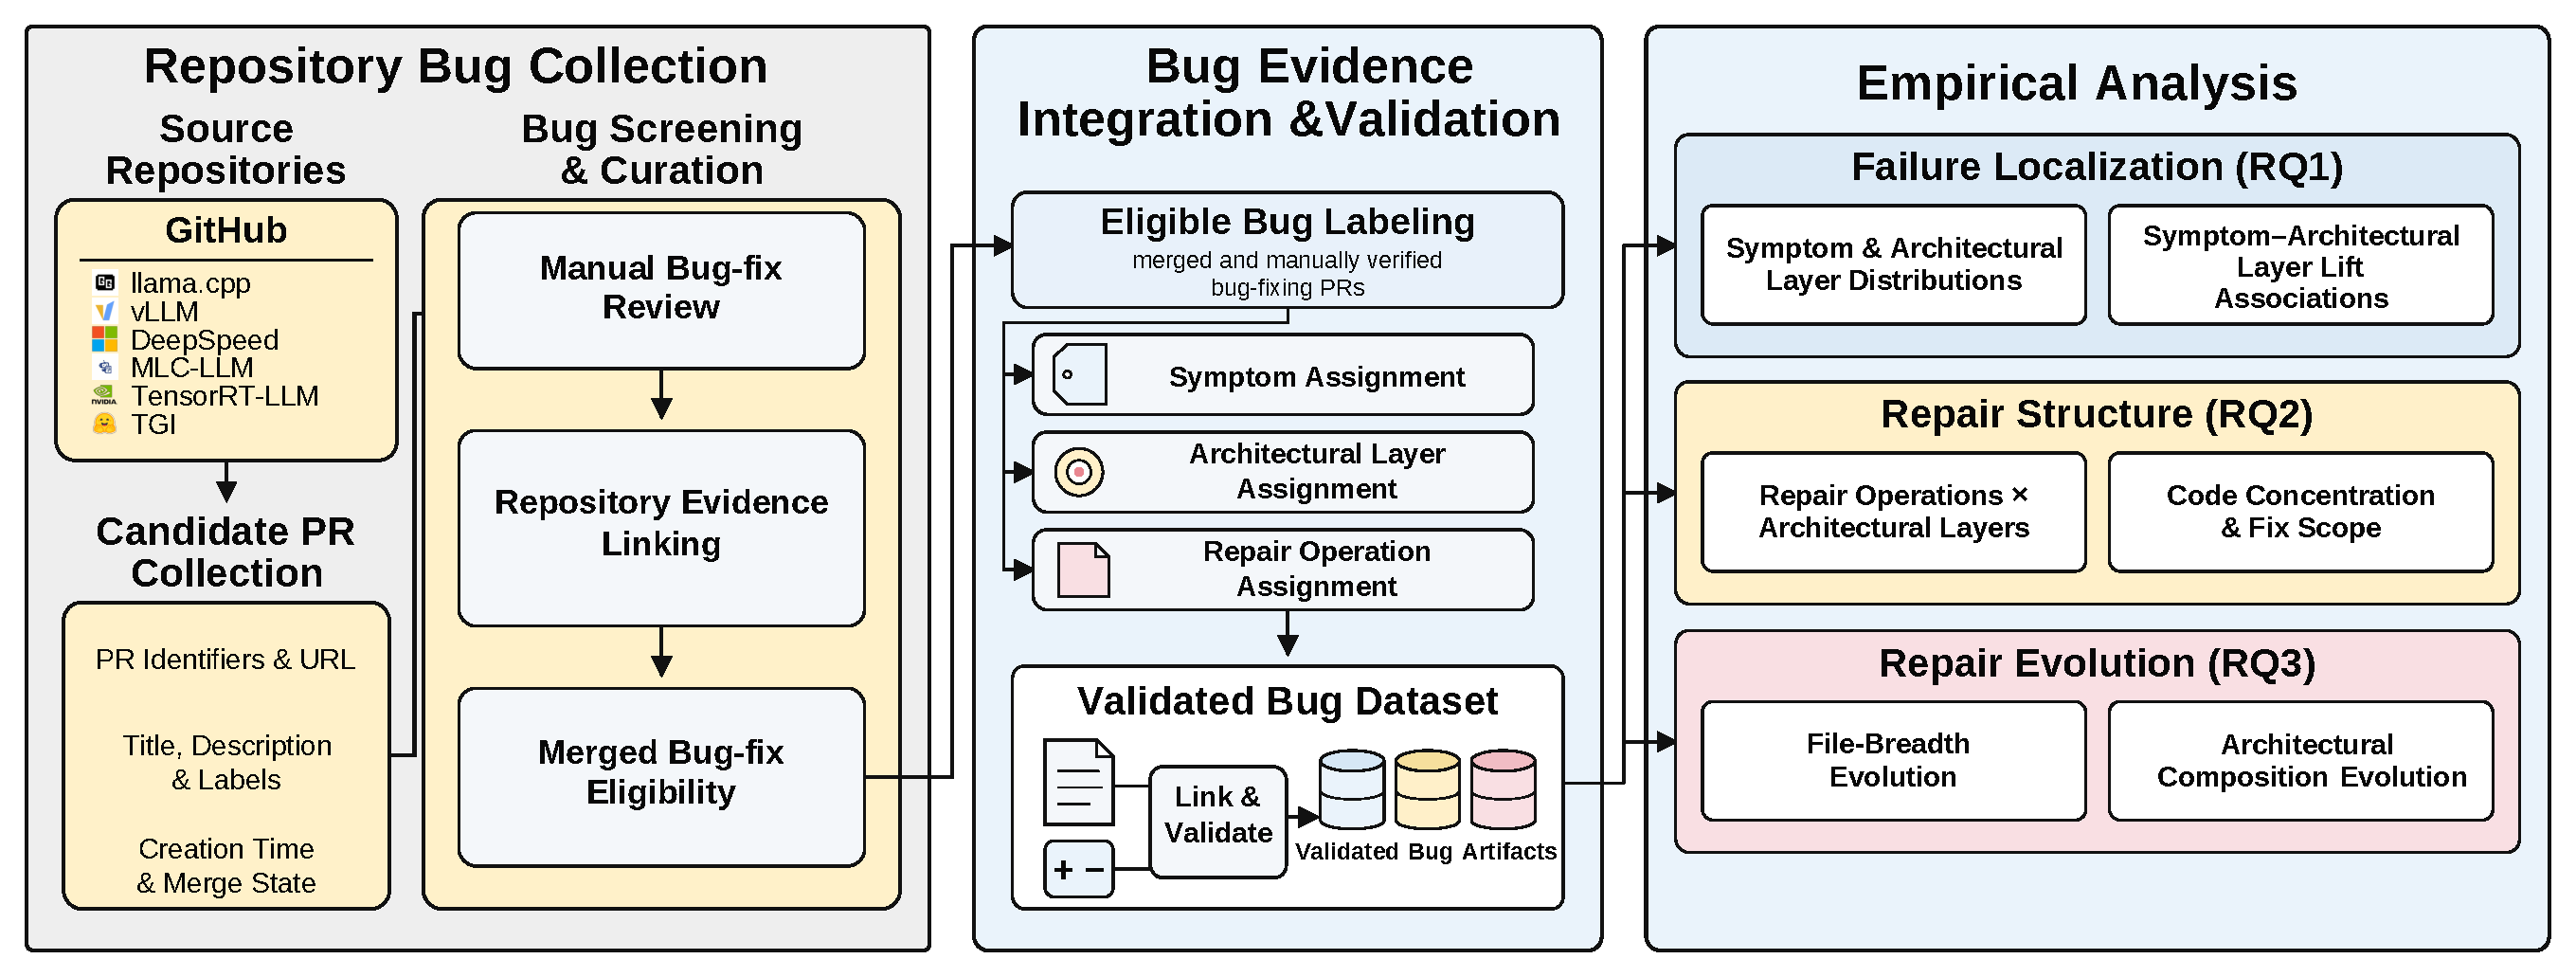
\includegraphics[width=\textwidth]{fig/workflow.pdf}
    \caption{Three-stage workflow of the empirical study: repository bug collection, bug-evidence integration and validation, and empirical analysis.}
    \label{fig:workflow}
\end{figure*}

\subsection{Repository Bug Collection}

\textbf{Source Repositories.} We study six widely used open-source engines for LLM inference: llama.cpp, vLLM, DeepSpeed, MLC-LLM, TensorRT-LLM, and Text Generation Inference (TGI). They represent the engine landscape surveyed in prior work~\cite{park2026inferenceengines} and cover local inference, high-throughput serving, compiler-based deployment, distributed execution, and hardware-specific acceleration. We use each project's official GitHub repository and include PRs from its earliest available records through March 2026. Table~\ref{tab:bug_stats} reports the period covered for each repository.

We collected 50,121 candidate bug-fixing PRs from the six repositories. For each PR, we recorded its repository and PR identifiers, URL, title, description, labels, and creation time. We did not rely solely on GitHub's bug labels because they are incomplete and may misclassify changes~\cite{bird2009mininggit,herzig2013misclassification}.


\begin{table}[t]
  \centering
  \caption{Study corpus by project.}
  \label{tab:bug_stats}
  \begin{tabular}{l c r r}
    \toprule
    Engine & Time frame & \# Candidates & \# Fixes \\
    \midrule
    llama.cpp    & Mar. 2023--Mar. 2026 & 10,549 & 3,004 \\
    vLLM         & Feb. 2023--Mar. 2026 & 23,561 & 5,915 \\
    DeepSpeed    & Jan. 2020--Mar. 2026 &  3,683 & 1,118 \\
    MLC-LLM      & Apr. 2023--Mar. 2026 &  1,816 &   487 \\
    TensorRT-LLM & Aug. 2023--Mar. 2026 &  8,802 & 1,784 \\
    TGI          & Oct. 2020--Mar. 2026 &  1,710 &   399 \\
    \midrule
    \textbf{Total} & --- & \textbf{50,121} & \textbf{12,707} \\
    \bottomrule
  \end{tabular}
\end{table}

\textbf{Bug Screening \& Curation.} Two experts with LLM inference-engine development experience independently reviewed each candidate PR. They examined the PR title and description, development discussion, linked issue, and complete patch to determine whether the change repaired an actual software defect. A PR was considered bug-fixing only when its evidence and patch established that it corrected unintended behavior; feature additions and other changes without evidence of defect correction were rejected. The experts discussed every disagreement until reaching consensus.

We linked each collected PR record to its development discussion, linked issue when available, complete patch, and GitHub merge state. We then combined these artifacts with the consensus screening decision, producing a traceable evidence record for each candidate rather than treating a repository label or PR description as sufficient evidence on its own.

The final corpus retains a PR only when it was both confirmed as bug-fixing through the review above and merged into the corresponding project codebase. This procedure produced 12,707 merged and manually verified bug-fixing PRs, distributed across the six projects as shown in Table~\ref{tab:bug_stats}.
\subsection{Bug Evidence Integration \& Validation}

\textbf{Eligible Bug Labeling.} The labels needed by our RQs cannot be recovered reliably from repository metadata alone. Symptoms describe externally observed failures, whereas architectural layers and repair operations require interpreting the development discussion together with the patch. We therefore derived the coding scheme directly from the collected PR evidence instead of treating GitHub labels as ground truth.

The two experts first reviewed an initial set of 1,000 PRs and used iterative open coding, following established guidance for qualitative empirical software-engineering research~\cite{seaman1999qualitative}, to derive candidate categories. They compared the proposed categories, discussed their boundaries, and repeatedly merged, split, or refined them when a category was ambiguous or failed to distinguish technically different cases. This process continued until the coding scheme stabilized, yielding ten symptom categories, nine architectural-layer categories, and nine repair-operation categories. The resulting taxonomies are grounded in recurring evidence from real fixes while retaining a common vocabulary applicable across all engines.

We assign one \emph{symptom} to each bug, representing the primary failure visible to a user or developer before the repair. We assign one \emph{repair operation}, representing the principal corrective action performed by the patch. Architectural-layer assignment is multi-label because a defect may span several architectural regions; accordingly, each bug is assigned one or more \emph{architectural layers} containing the faulty logic or state responsible for the failure. Architectural-layer labels identify faulty locations rather than indiscriminately treating every file modified by a patch as a fault location.

After the taxonomies were finalized, the two experts independently applied them to the complete corpus. Each decision was based on the same evidence used for eligibility review: the PR description, discussion, linked issue, and complete patch. They then compared their labels and resolved disagreements through discussion until consensus.

\textbf{Evidence Integration.} For each verified fix, this stage combines repository metadata, development discussion, linked issues when available, the complete patch, and the consensus labels produced through the labeling procedure above. We link these artifacts by repository and PR identifier and consolidate them into one structured record per fix. Each record preserves the PR URL and creation time, the evidence used during review, one symptom, one repair operation, one or more architectural layers, and the patch metadata required to measure modified entities and fix scope.

\textbf{Record Validation.} We validate each integrated record against the eligibility decision established during screening and the consensus labels produced through the labeling procedure above. In particular, the record must refer to a merged PR, carry the consensus bug-fixing decision and required labels, and link to the patch reviewed by the experts. The resulting analysis-ready dataset contains 12,707 validated records. Architectural layers are retained as a list within a single bug record rather than expanded into duplicate rows; the weighting or expansion required by a particular analysis is applied explicitly in the next stage. This preserves a stable denominator while allowing RQ1 and RQ2 to use different multi-layer counting rules.
%The collection stage produces several artifacts for each verified fix: repository metadata, development discussion, linked issues when available, the complete patch, and consensus labels. We link these artifacts by repository and PR identifier and consolidate them into one structured record per fix. Each record preserves the PR URL and creation time, the evidence used during review, one symptom, one repair operation, one or more architectural layers, and the patch metadata required to measure modified entities and fix scope.

%We validate the integrated record against the evidence and eligibility decisions established in the previous stage. In particular, the record must refer to a merged PR, carry the consensus bug-fixing decision and required labels, and link to the patch reviewed by the experts. The resulting dataset contains 12,707 validated records. Root-cause layers are retained as a list within a single bug record rather than expanded into duplicate rows; the weighting or expansion required by a particular analysis is applied explicitly in the next stage. This preserves a stable denominator while allowing RQ1 and RQ2 to use different multi-layer counting rules.


\subsection{Empirical Analysis}

The final stage answers the three research questions through complementary analyses. RQ1 relates externally observed symptoms to the architectural layers containing the faulty code. RQ2 characterizes how repairs are structured across repair operations, architectural layers, and code entities. RQ3 tracks how repair scope evolves over time.

\textbf{Failure Localization (RQ1).} To characterize where failures manifest and where their underlying faults reside, we compute the distributions of symptoms and architectural layers for each project and for the combined corpus. Because a bug may have multiple architectural layers, counting it once in every assigned layer would give multi-layer bugs disproportionate influence. We therefore assign a weight of $1/k$ to each of a bug's $k$ architectural layers, keeping the bug's total weight at one.

We quantify the association between a symptom $s$ and an architectural layer $l$ using lift. Let $w_{s,l}$ be the weighted number of bugs having symptom $s$ and layer $l$, $w_s$ the total weight of bugs with symptom $s$, $w_l$ the total weight assigned to layer $l$, and $W$ the total weight of all verified bugs. We compute
\begin{equation}
    \operatorname{Lift}(s,l)
    = \frac{P(l\mid s)}{P(l)}
    = \frac{w_{s,l}/w_s}{w_l/W}.
\end{equation}
A lift greater than one indicates that layer $l$ is overrepresented among bugs with symptom $s$ relative to its prevalence in the full corpus; a value below one indicates underrepresentation. We use lift as a descriptive association measure and do not interpret it as evidence of causality.

\textbf{Repair Structure (RQ2).} We characterize how bug-fixing work is structured across architectural layers and code entities from three complementary perspectives. First, we cross-tabulate repair operations with architectural layers. Although each bug has exactly one repair operation, a bug assigned to $k$ architectural layers contributes one repair-operation instance to each of those layers. Consequently, the 12,707 fixes yield 19,965 repair-operation instances. This rule includes every affected layer in the repair-operation counts.

Second, we measure code concentration at file and function granularity. Prior work has shown that fault-prone locations and change history are useful signals for focusing quality-assurance effort~\cite{ostrand2005faultlocation,graves2000changehistory}. For each project, we count the bug-fixing occurrences associated with each entity, rank entities in descending order, and construct cumulative concentration curves. We report the fraction of all bug-fixing occurrences covered by the top 20\% of files and functions, as well as the fraction of entities required to cover 80\% of the occurrences.

Third, we quantify the scope of each fix using changed lines and modified files. Changed lines are the sum of added and deleted lines in the complete PR patch, whereas the number of modified files captures how broadly the repair spreads across the repository. These change-level measures are consistent with prior just-in-time quality-assurance research that treats properties of individual changes as review and testing signals~\cite{kamei2013jitqa}. They describe repair scope rather than bug severity. Because fix sizes are strongly right-skewed, we characterize their distribution using the median and upper quantiles instead of relying on the mean. For RQ3, we pair these patch-level measures with layer-level fix distributions.

Because their units differ, we keep the three RQ2 measures separate. Repair-operation instances count actions in each affected layer; entity concentration records repeated changes to files and functions; changed lines and modified files describe a complete fix. A combined score would blur important distinctions: a large patch is not necessarily severe, a frequently modified entity is not faulty in every PR, and a multi-layer fix is not several independent bugs.

\textbf{Repair Evolution (RQ3).} To examine how repair scope evolves over time, we group fixes by the month when their PR was created. Several projects have few monthly observations before 2023, so the trend analysis covers January 2023 through March 2026. For each month, we group fixes by the number of modified files---one file, two to five files, or at least six files---and track the share of each group. We also track the share of bug-fixing activity in each architectural layer. We first remove duplicate layer labels for each bug. We then split its weight equally among those layers, keeping the total at one.

To test whether each monthly layer share generally increases or decreases over time, we compute Spearman's rank correlation between the month number and the layer share. Let $t\in\{1,\ldots,n\}$ be the month number, where $n=39$, and let $Y_t$ be the weighted share of a layer in month $t$. If $R_t$ is the rank of month $t$ and $S_t$ is the rank of $Y_t$, with average ranks for tied values, the correlation is
\begin{equation}
\rho =
\frac{\sum_{t=1}^{n}(R_t-\bar{R})(S_t-\bar{S})}
{\sqrt{\sum_{t=1}^{n}(R_t-\bar{R})^2}
 \sqrt{\sum_{t=1}^{n}(S_t-\bar{S})^2}}.
\label{eq:spearman_temporal}
\end{equation}
A positive $\rho$ indicates that the layer's monthly share tends to increase over time, whereas a negative value indicates that it tends to decrease. We use Spearman's correlation because it can capture a general upward or downward trend without assuming a straight-line relationship or a normal distribution of monthly values. For each layer, we obtain a two-sided $p$-value for the null hypothesis $H_0:\rho=0$ using 20,000 random permutations. Because we test nine architectural layers, some trends may appear significant by chance. We therefore apply the Benjamini--Hochberg procedure~\cite{benjamini1995controlling} to the nine $p$-values, control the false discovery rate---the expected share of false positives among trends declared significant---at 0.05, and report the adjusted values as $q$-values. We also report the least-squares slope in percentage points per year to make the size of each change easier to understand.

To check whether an overall trend is caused by changes in the mix of projects, we recompute the monthly layer shares for each project and combine them using fixed project weights based on the full analysis period. When a project has no fixes in a month, we adjust the weights of the active projects so that they still sum to one. Because we use the PR creation date, this analysis shows how observed bug-fixing activity changes over time. It does not measure when bugs were introduced, how long they took to discover, or how long they took to repair.

\section{Empirical Results}
\subsection{RQ1: Failure Localization}
To answer RQ1, we first examine the distribution of externally observable symptoms across the six inference engines. We then locate the faulty code in nine architectural layers and analyze the association between symptoms and architectural layers. When a bug spans multiple architectural layers, its unit weight is divided equally among those layers so that each bug contributes a total weight of one.
\newcommand{\findbox}[2][]{%
  \noindent
  \begin{tcolorbox}[
    arc=2pt,
    boxrule=0.4pt,
    colback=white,
    colframe=black,
    left=1mm,
    right=1mm,
    top=0.8mm,
    bottom=0.8mm,
    width=\linewidth,
    before skip=2pt,
    after skip=2pt,
    fontupper=\normalsize,
    #1,
  ]
  #2
  \end{tcolorbox}
  \par
}

\begin{figure}[!b]
    \centering
    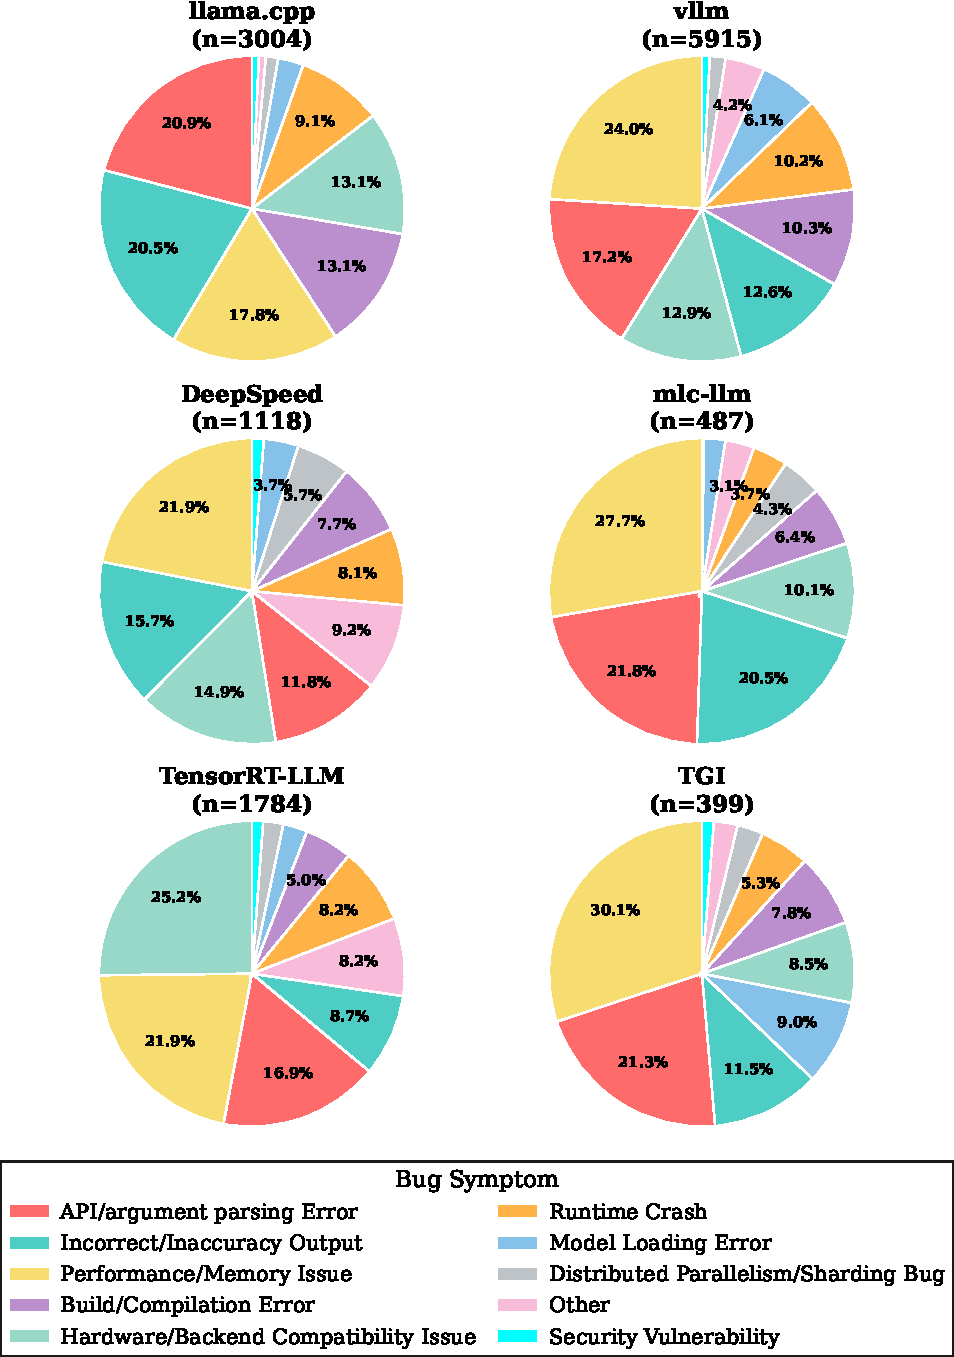
\includegraphics[width=\linewidth]{fig/symptom_distribution_by_project.pdf}
    \caption{Bug-symptom distributions across six inference engines.}
    \label{fig:symptom_dist}
\end{figure}
% \noindent\hspace*{2em}

\noindent\textbf{Observable Symptom Analysis.} As shown in Fig.~\ref{fig:symptom_dist}, we compare how bugs become externally visible across the six inference engines. Together, these distributions reveal which failure manifestations dominate among the studied fixes and which symptoms deserve greater attention in testing.

% \textbf{Critical correctness and availability failures remain common.}
% Figure~\ref{fig:symptom_dist} reveals two common properties of the symptom distributions. 
First, symptoms that threaten correctness and availability constitute a substantial portion of the maintenance burden. Incorrect outputs, runtime crashes, and model-loading failures collectively account for 4,001 of the 12,707 studied bugs (31.5\%), ranging from 23.6\% to 35.6\% across individual engines. This recurring presence matters because the three symptoms expose different detection challenges. Crashes and loading failures usually provide explicit failure signals, whereas incorrect outputs may pass through the serving pipeline without an obvious error. Bug detection should therefore combine conventional crash and initialization checks with output oracles, differential testing, and validation of intermediate execution states. For developers, the result also suggests that regression suites should exercise the complete path from model loading to execution and output validation rather than treating successful startup or request completion as proof of correctness.


% \noindent\hspace*{2em}\textbf{A few symptoms dominate each engine.}
Second, the overall symptom distribution is consistently top-heavy: each engine's three most frequent symptoms account for 52.5\%--70.0\% of its bugs. Because this concentration appears in every project, it is unlikely to be merely an artifact of the largest repositories. The result provides a practical basis for prioritization: project-specific tests, monitors, and bug triage rules targeting a small set of recurrent symptoms can cover a substantial share of historically observed failures. However, the variation in both concentration strength and symptom composition cautions against adopting one global testing profile for all engines. Teams should derive priorities from their own engine's failure history and retain broader checks for the long tail, since even the most concentrated project leaves 30.0\% of bugs outside its top three categories.


% \noindent\hspace*{2em}\textbf{The dominant symptom differs with project emphasis.}
API/argument-parsing errors form the largest category in four engines. They account for 24.0\% of vLLM bugs and 21.9\% of those in DeepSpeed. The corresponding shares rise to 27.7\% in MLC-LLM and 30.1\% in TGI. A different pattern appears in the other two projects. Incorrect outputs lead in llama.cpp and represent 20.9\% of its bugs, whereas 25.2\% of TensorRT-LLM bugs concern performance or memory, making this its most frequent symptom. These profiles are consistent with the different technical surfaces exposed by the projects. Server-oriented engines maintain extensive APIs and configuration paths, llama.cpp emphasizes portable inference across models and platforms, and TensorRT-LLM aggressively targets hardware-specific throughput and memory efficiency. This interpretation explains a plausible correspondence between project emphasis and observed symptoms, but the descriptive data do not establish a causal relationship.
% Finding #1
\findbox{\textbf{Finding \#1:} Bug symptoms concentrate in a few categories across all six engines, but the leading categories differ by project. Incorrect outputs, runtime crashes, and model-loading failures together account for 31.5\% of the corpus; each project's three most frequent symptoms cover 52.5\%--70.0\% of its bugs.}

\begin{figure}[htbp]          % 去掉 *，改为单栏 figure
    \centering
    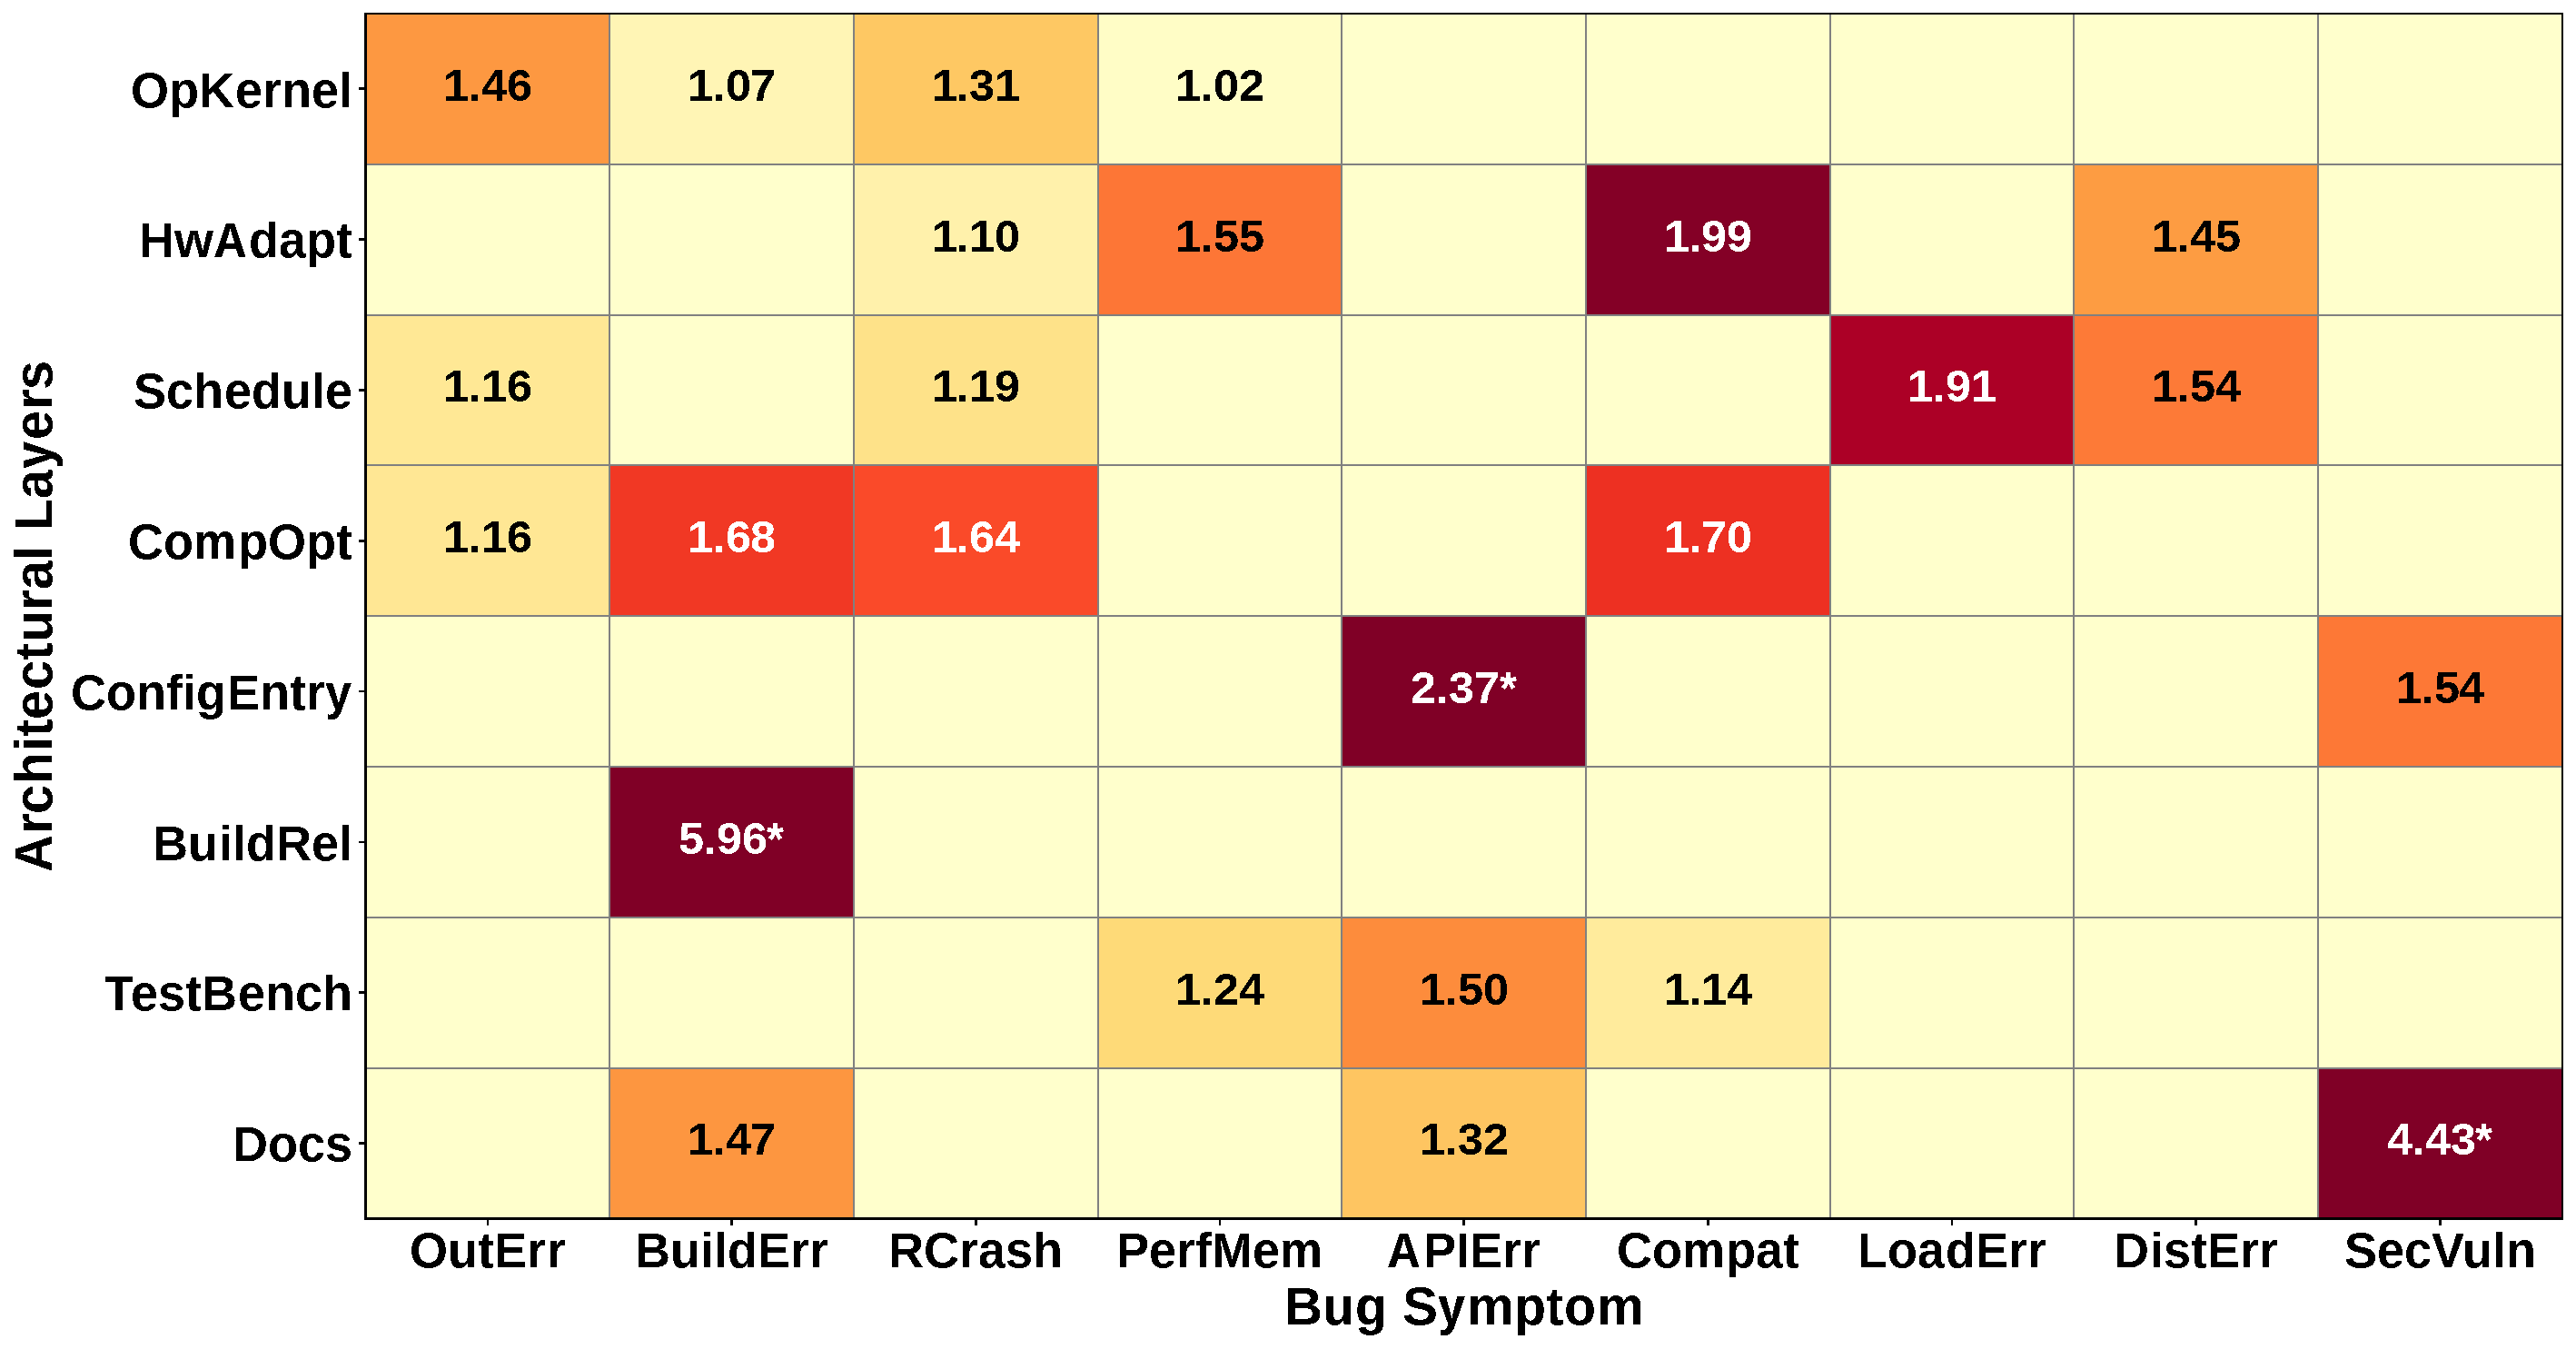
\includegraphics[width=0.95\columnwidth]{fig/root_cause_symptom_lift_heatmap_range_1_2.pdf}
    \caption{Lift of associations between architectural layers and bug symptoms across six LLM inference engines. Values above one mean that a symptom appears more often in a layer than in the full corpus.}
    \label{fig:symptom_arch_layer_lift_heatmap}
\end{figure}
\noindent\textbf{Bug Symptoms Across Architectural Layers.}
Figures~\ref{fig:symptom_arch_layer_lift_heatmap} and~\ref{fig:symptom_distribution_by_arch_layer} expose a markedly uneven relationship between symptoms and architectural layers. Relating the two dimensions reveals which symptoms are more strongly associated with particular architectural layers. Rather than sharing a common symptom distribution, several specialized layers exhibit a distinctive failure signature consistent with their role.


Bugs in Build/Release and Config/Entrypoint are each dominated by one symptom category. Build and compilation errors represent 86.1\% of the weighted bugs in Build/Release and yield the highest observed lift of 5.96. API and argument parsing errors make up 53.0\% of Config/Entrypoint bugs. This symptom is 2.37 times as common in Config/Entrypoint as it is across the full corpus. These profiles give developers focused starting points for diagnosis. Compilation failures direct attention toward dependency specifications, build scripts, and continuous integration environments, while input related failures point toward configuration schemas, request validation, and entrypoint logic. Build matrices and systematic input validation can expose such faults before deployment, while records of resolved configurations can shorten diagnosis when the visible error does not identify its source.

% \noindent\hspace*{2em}\textbf{Hardware Adaptation exposes both compatibility and efficiency problems.}
Hardware Adaptation has a broader symptom profile, yet compatibility and efficiency problems remain prominent. Hardware and backend compatibility issues account for 19.4\% of its weighted bugs and occur at nearly twice the rate expected from the full corpus. Performance and memory issues form an even larger share at 22.6\%. This combination reflects the dual responsibility of hardware specific code, which must preserve functional interoperability while using devices efficiently. Testing this layer should therefore vary devices, drivers, and precision settings while checking both output correctness and resource behavior. Taken together, the three specialized layers show that architectural responsibility influences how faults become visible. Their characteristic symptoms can narrow the initial search area, although they should guide diagnosis rather than determine it.




\begin{figure}[htbp]          % 去掉 *，改为单栏 figure
    \centering
    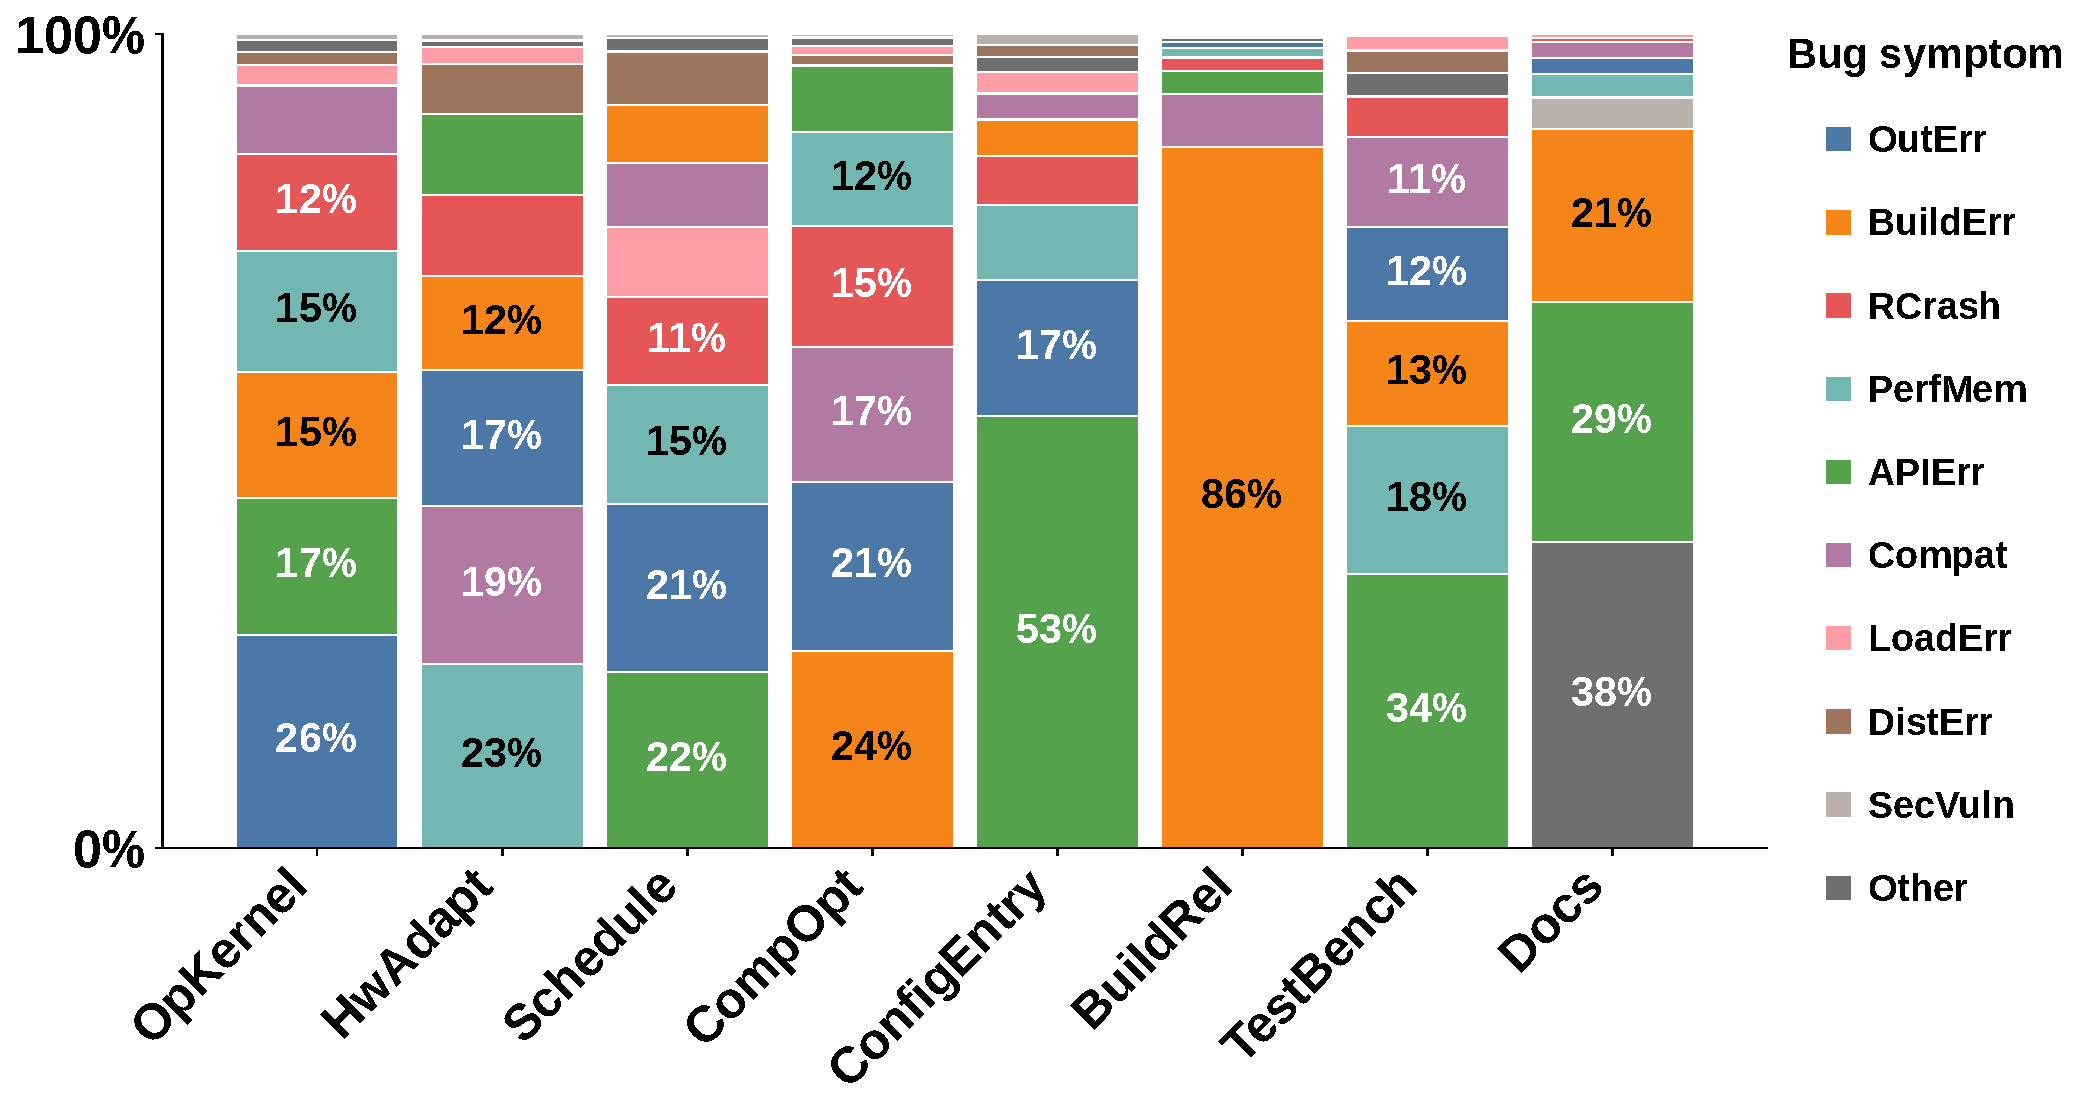
\includegraphics[width=0.95\columnwidth]{fig/root_cause_symptom_stacked_percentage.pdf}
    \caption{Distribution of bug symptoms within each architectural layer across six LLM inference engines.}
    \label{fig:symptom_distribution_by_arch_layer}
\end{figure}
% Finding #2
\findbox[before skip=6pt,after skip=0pt]{\textbf{Finding \#2:} Symptom profiles vary systematically across architectural layers. In particular, Build/Release, Config/Entrypoint, and Hardware Adaptation exhibit narrow failure signatures aligned with their roles, so their characteristic symptoms can guide initial localization.}

% \noindent\textbf{}

Scheduler/Runtime illustrates why a frequent layer is not necessarily easy to diagnose. It contains 38.5\% of the weighted bugs, yet no symptom accounts for one quarter of them. API and argument parsing errors lead at only 21.6\%, closely followed by incorrect outputs at 20.7\%. The remaining failures include performance problems, crashes, and failures involving loading or distributed execution. This diversity is consistent with the coordinating role of scheduler and runtime code. A single request may depend on admission and batching, model and memory state, and distributed worker execution before producing a result. Faults in any of these interactions can therefore converge on similar external symptoms. Monitoring only final outcomes provides little evidence about where the failure began. Developers need stage level telemetry that records queue transitions, cache state, and distributed worker events across the request lifetime.

Compiler/Optimization accounts for only 3.4\% of the weighted corpus but shows a similarly broad profile. Build and compilation errors form its largest category at 24.2\%, while incorrect outputs follow closely at 20.8\%. Another 16.6\% appear as hardware or backend compatibility problems. These outcomes show that an optimization fault does not always stop compilation. An invalid transformation may instead generate a numerically incorrect kernel, fail only on a particular backend, or alter runtime resource use. A successful build is therefore a weak oracle for this layer. Tests should compare optimized and unoptimized execution, inspect intermediate representations, and validate results across backend and precision settings.

The contrast with Finding~\#2 lies in diagnostic specificity rather than bug frequency alone. A build or parsing error can substantially narrow the likely search area. Crashes, incorrect outputs, and performance regressions provide weaker guidance because several interacting execution layers can produce them. Effective diagnosis in Scheduler/Runtime and Compiler/Optimization must connect the final symptom with runtime traces, intermediate states, and backend comparisons. Tests that span model preparation, request execution, and device execution are also needed to reveal failures that emerge only through cross layer interactions.

% Finding #3
\findbox{\textbf{Finding \#3:} In contrast to specialized boundary layers, Scheduler/Runtime and Compiler/Optimization produce broad, overlapping symptom profiles. Their faults cross correctness, availability, performance, and compatibility boundaries, making symptom-only localization substantially less reliable.}

\begin{table}[t]
    \centering
    \caption{Definitions of repair operations.}
    \label{tab:repair_operations}
    \renewcommand{\arraystretch}{1.3}
    \setlength{\tabcolsep}{3pt}
    \begin{tabular}{p{0.22\columnwidth} p{0.63\columnwidth} c}
        \toprule
        \textbf{Operation} & \multicolumn{1}{c}{\textbf{Description}} & \textbf{ID} \\
        \midrule
        Logic Correction & Fixes logical errors, calculations, conditions, or state transitions. & (Cor) \\
        Adaptation & Adjusts for different hardware, platforms, APIs, or compatibility. & (Adp) \\
        Configuration & Modifies runtime options, default parameters, or feature flags. & (Cf) \\
        Validation & Adds checks to reject invalid inputs, states, permissions, or preconditions. & (Val) \\
        Reorganization & Restructures data structures, control flow, or module interactions. & (Rg) \\
        Recovery & Enhances failure handling, rollbacks, retry, or fallback mechanisms. & (Rv) \\
        Optimization & Improves performance/memory efficiency without behavioral changes. & (Opt) \\
        Synchronization & Adjusts ordering or coordination across threads, devices, or processes. & (S) \\
        Allocation & Changes memory, buffer, cache, or resource allocation and release. & (Al) \\
        \bottomrule
    \end{tabular}
\end{table}

\subsection{RQ2: Repair Structure}

RQ2 examines repair structure through repair operations, code entity concentration, and fix scope. Each fix is assigned one of the nine repair operations defined in Table~\ref{tab:repair_operations}. Fifteen fixes with rare residual operations are grouped as Other and excluded from the operation analysis. When a fix spans multiple architectural layers, its operation contributes one instance to each assigned layer. The resulting 19,965 instances describe layer participation rather than unique fixes.

Code entity concentration is measured separately for files and functions. Fix scope is measured with changed lines and modified files, which capture the amount and breadth of code modification. Complete diffs are available for all 12,707 fixes. Since changed lines are strongly skewed, we use the median and upper quantiles instead of the mean. The median is 14 lines, while P75, P90, and P95 reach 52, 165, and 326.7 lines.


\noindent\textbf{Code Entity Concentration.}
The resulting concentration profiles show where bug-fixing activity has historically accumulated and which code entities may warrant closer attention. Figure~\ref{fig:file_function_concentration} shows that bug fixes are concentrated in a limited portion of the codebase. The top 20\% of files account for 79.6\% of weighted bug associations, while the same fraction of functions accounts for 68.4\%. This difference suggests that maintenance repeatedly returns to a small group of modules but spans several implementation units in each. File histories can therefore identify modules that deserve early attention, while function histories provide a finer search space for diagnosis and review.

The pattern persists in every engine rather than being produced by one large repository. Depending on the project, the top 20\% of files cover between 69.3\% and 85.1\% of weighted bug associations. Function coverage ranges from 61.7\% to 69.4\%. These recurring concentrations support a staged quality assurance strategy. Teams can use file histories to prioritize risky modules, then use function histories to focus regression testing, review, and refactoring.

\findbox{\textbf{Finding \#4:} Bugs are strongly concentrated in a small set of files and functions. The top 20\% of files account for 79.6\% of weighted bug associations, while the top 20\% of functions account for 68.4\%.}

\begin{figure}[t]
    \centering
    \subfloat{%
        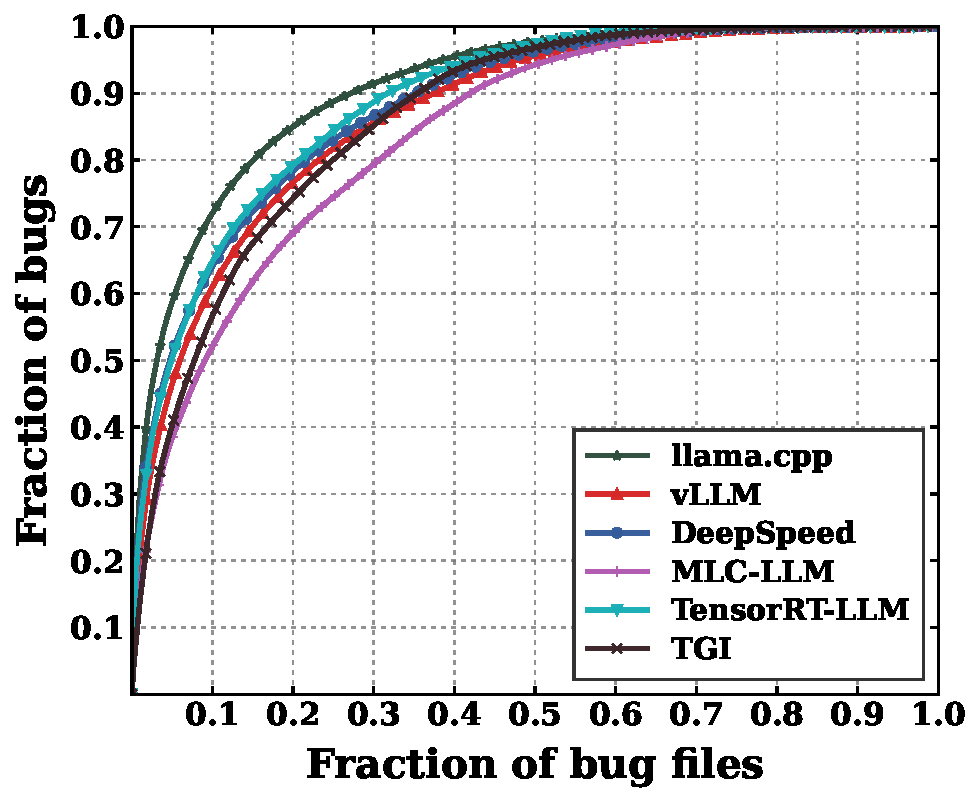
\includegraphics[width=0.49\columnwidth]{fig/concentration_curve_files_weighted_alpha0.8_by_project_multi_project.pdf}%
    }\hfill
    \subfloat{%
        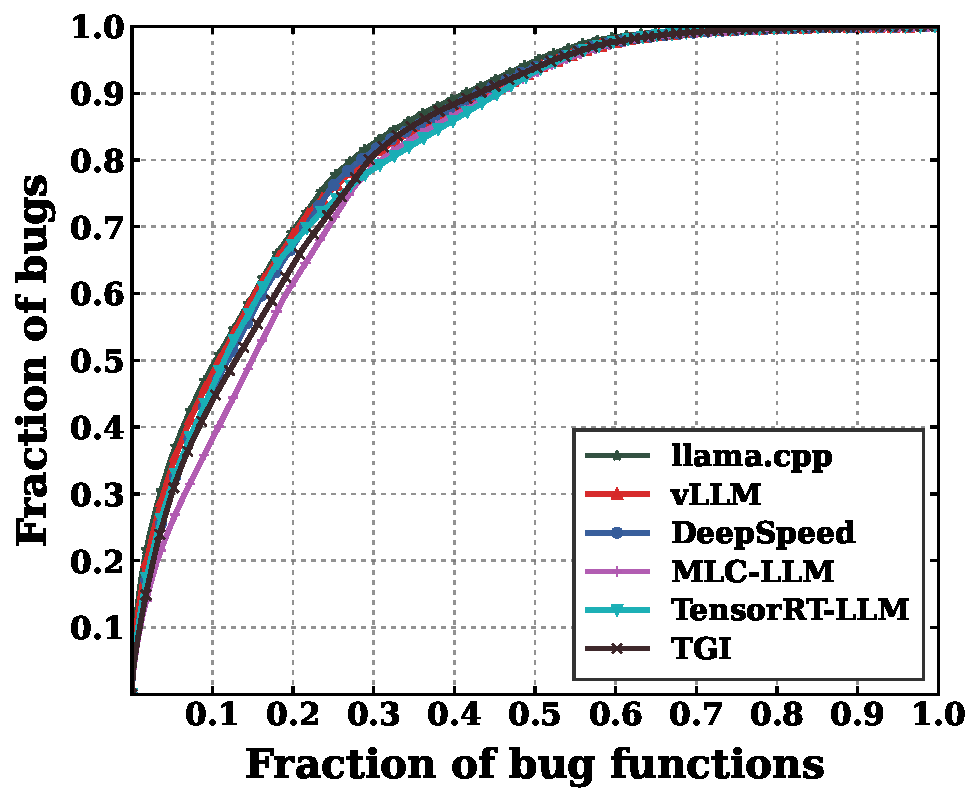
\includegraphics[width=0.49\columnwidth]{fig/concentration_curve_functions_weighted_alpha0.8_by_project_multi_project.pdf}%
    }
    \caption{Per-project bug concentration curves at file and function granularity. Entities are ranked in descending order by their associated bug counts. The x-axis represents the cumulative fraction of files or functions, and the y-axis represents the cumulative fraction of bugs.}
    \label{fig:file_function_concentration}
\end{figure}

\noindent\textbf{Repair Operation Distribution.}
Examining this distribution reveals which forms of code change dominate maintenance and how their prevalence varies across architectural layers. Table~\ref{tab:repair_counts} shows that Logic Correction and Adaptation account for 14,702 of the 19,965 repair operation instances, or 73.6\%. Their dominance shows that much of the maintenance workload addresses faulty program behavior or adapts the engine to changing execution environments. Review and testing should therefore pay particular attention to state transitions, compatibility assumptions, and behavior across supported platforms. The concentration also suggests that repair tools designed around these recurring operations could assist a substantial portion of observed fixes without assuming that all layers fail in the same way.

The two operations remain prevalent across most of the architecture. Their combined share exceeds 65\% in seven of the eight principal layers and reaches 80.5\% in Compiler/Optimization. Build/Release is the exception. Logic Correction and Adaptation account for 46.7\% of its instances, while Configuration alone contributes 43.2\%. This distinct profile reflects the role of build scripts, dependency specifications, and packaging settings. It also indicates that maintenance support for this layer should emphasize configuration validation rather than relying only on techniques aimed at program logic or platform adaptation.

\findbox{\textbf{Finding \#5:} Repair operations exhibit a highly concentrated distribution. Logic Correction and Adaptation dominate the overall maintenance workload and remain prevalent across most architectural layers.}

\begin{table}[t]
    \centering
    \caption{Architectural layer \(\times\) repair operation counts.}
    \label{tab:repair_counts}
    \resizebox{\linewidth}{!}{%
        \begin{tabular}{l c c c c c c c c c}
            \toprule
            \diagbox[width=2.4cm, height=0.6cm]{\textbf{Layer}}{\raisebox{0pt}{\hspace{1.25cm}\textbf{Operation}}}
            & \textbf{Corr.} & \textbf{Adapt.} & \textbf{Config.} & \textbf{Valid.} & \textbf{Reorg.} & \textbf{Recov.} & \textbf{Optim.} & \textbf{Sync.} & \textbf{Alloc.} \\[-0.18cm]
            & (Cor) & (Adp) & (Cf) & (Val) & (Rg) & (Rv) & (Opt) & (S) & (Al) \\[+0cm]
            \midrule
            Scheduler/Runtime & 3816 & 2305 & 239 & 515 & 450 & 228 & 228 & 163 & 35 \\
            Hardware Adapt. & 1477 & 1495 & 126 & 179 & 182 & 131 & 123 & 123 & 81 \\
            Operators/Backend & 1279 & 746 & 81 & 206 & 147 & 69 & 67 & 38 & 43 \\
            Config/Entrypoint & 896 & 442 & 187 & 231 & 158 & 61 & 29 & 29 & 6 \\
            Tests/Bench & 648 & 560 & 321 & 111 & 87 & 67 & 11 & 25 & 9 \\
            Compiler/Optim. & 314 & 267 & 29 & 31 & 17 & 10 & 39 & 11 & 4 \\
            Build/Release & 102 & 143 & 227 & 15 & 31 & 5 & 0 & 2 & 0 \\
            Docs & 196 & 16 & 53 & 1 & 0 & 2 & 0 & 0 & 0 \\
            \bottomrule
        \end{tabular}%
    }
\end{table}



\subsection{RQ3: Repair Evolution}
For RQ3, we track how bug-fixing activity changes over time in both repair scope and architectural distribution. The analysis includes 12,707 pull requests with complete diffs and valid timestamps from February 2020 to March 2026. Monthly observations are sparse during the early development of several projects, so the formal trend analysis covers the 12,299 fixes created between January 2023 and March 2026.

Modified files measure how broadly a fix spreads across the codebase. To examine whether the architectural focus of bug-fixing activity also changes, we compute the monthly weighted share of each architectural layer. Following RQ1, the layers assigned to a bug are first deduplicated, and a bug spanning $k$ layers contributes $1/k$ to each layer so that every bug has a total weight of one. We use Spearman's rank correlation to assess monotonic trends over the 39 monthly observations and apply the Benjamini--Hochberg procedure across the nine layer-level tests. Each observation is assigned to the creation month of its fixing pull request. The results therefore describe the evolution of observed bug-fixing activity rather than bug introduction time, discovery delay, or changes in the intrinsic reliability of an architectural layer.

\begin{figure}[t]
    \centering
    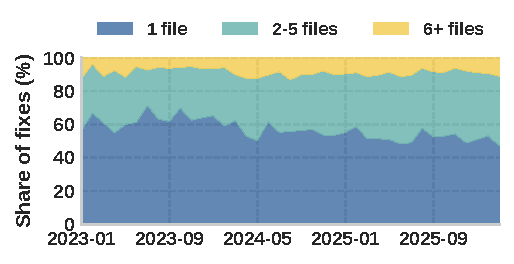
\includegraphics[width=\columnwidth]
        {fig/monthly_file_bucket_trend_single_column.pdf}
    \caption{Monthly distribution of bug fixes by the number of modified files from January 2023 to March 2026.}
    \label{fig:monthly-file-bucket-trend}
\end{figure}

\noindent\textbf{File Breadth Evolution.}
Tracking file breadth clarifies how widely fixes spread and whether repairs increasingly involve coordinated changes across multiple files. Figure~\ref{fig:monthly-file-bucket-trend} shows that single file fixes remain the largest category, but their share decreases from 56.3\% in January 2023 to 47.1\% in March 2026. Over the same period, fixes spanning two to five files rise from 31.3\% to 41.8\%. The similar size of these changes indicates that the main shift occurs from isolated modifications toward repairs requiring coordination across a small group of files. Developers should review connected changes together and test interactions among the modified components.

Fixes touching at least six files grow from 4 to 95 in monthly volume, yet their share changes from 12.5\% to 11.1\%. Their absolute workload increases as project activity expands, but they do not become more prevalent relative to other fixes. The evidence therefore indicates a broader routine repair surface, not a growing proportion of very large multi-file changes.

% Finding #6
\findbox{\textbf{Finding \#6:} Single-file fixes remain the largest category, but the repair mix shifts toward changes spanning two to five files. Fixes touching six or more files grow strongly in absolute volume without increasing their relative share.}

\begin{table}[t]
    \centering
    \caption{Weighted architectural-layer changes over time.}
    \label{tab:monthly-layer-trends}
    \scriptsize
    \setlength{\tabcolsep}{3pt}
    \resizebox{\columnwidth}{!}{%
    \begin{tabular}{lrrrrr}
        \toprule
        \textbf{Architectural layer} &
        \textbf{First 12m} &
        \textbf{Last 12m} &
        \boldmath$\Delta$ \textbf{(pp)} &
        \boldmath$\rho$ &
        \boldmath$\rho_{\mathrm{adj}}$ \\
        \midrule
        Hardware Adaptation      &  6.4\% & 23.7\% & $+17.2$ &  $0.781$ &  $0.739$ \\
        Tests/Bench              &  3.2\% & 12.5\% &  $+9.3$ &  $0.822$ &  $0.675$ \\
        Config/Entrypoint        &  4.9\% & 10.4\% &  $+5.5$ &  $0.564$ &  $0.239$ \\
        Compiler/Optimization    &  2.1\% &  4.0\% &  $+2.0$ &  $0.525$ &  $0.443$ \\
        \midrule
        Scheduler/Runtime        & 44.1\% & 33.6\% & $-10.5$ & $-0.382$ & $-0.668$ \\
        Docs                     &  2.8\% &  1.1\% &  $-1.7$ & $-0.576$ & $-0.154$ \\
        Operators/Backend        & 22.4\% &  9.1\% & $-13.3$ & $-0.654$ & $-0.156$ \\
        Other                    &  6.8\% &  3.7\% &  $-3.1$ & $-0.670$ & $-0.137$ \\
        Build/Release            &  7.2\% &  1.9\% &  $-5.3$ & $-0.789$ & $-0.645$ \\
        \bottomrule
    \end{tabular}
    }
    \vspace{2pt}

    \begin{minipage}{\columnwidth}
        \scriptsize
        \emph{Notes:} ``First'' and ``Last'' are mean monthly shares; $\Delta$ is their difference in percentage points. $\rho$ is the pooled Spearman correlation and $\rho_{\mathrm{adj}}$ uses fixed project weights. Here, $q$ denotes the Benjamini--Hochberg-adjusted $p$-value. All pooled trends remain significant after correction ($q\leq0.0011$), except Scheduler/Runtime ($q=0.017$).
    \end{minipage}
\end{table}

\noindent\textbf{Architectural Composition Evolution.}
The layer trends in Table~\ref{tab:monthly-layer-trends} show that the architectural distribution of bug-fixing activity changes substantially over the study period. Hardware Adaptation exhibits the clearest increase. Its monthly weighted share has a strong positive association with time ($\rho=0.781$, $p<0.001$), rising from an average of 6.4\% during the first 12 months of the analysis window to 23.7\% during the last 12 months. This difference of 17.2 percentage points is also reflected in an estimated increase of 7.3 percentage points per year. After correcting for the nine layer-level comparisons, the trend remains statistically significant ($q<0.001$).

This result is not explained solely by the changing contribution of the six projects. A project-standardized monthly series, constructed using fixed analysis-window project weights, retains a strong positive association ($\rho=0.739$) and an estimated increase of 6.6 percentage points per year. The direction is also positive within several engines, with particularly clear increases in llama.cpp, TGI, and vLLM. Together, these observations indicate that the growing share of Hardware Adaptation fixes reflects a recurring cross-project shift rather than only the expansion of one repository.

Tests/Bench also increases in the pooled data ($\rho=0.822$, $p<0.001$), from 3.2\% in the first 12 months to 12.5\% in the last 12 months. Unlike Hardware Adaptation, however, this pattern is driven primarily by vLLM and is nearly flat in most other projects. We therefore treat it as a project-dependent trend rather than evidence of a common architectural shift across inference engines.

Because the monthly layer shares sum to 100\%, these trends describe a change in composition. An increase in one layer necessarily coincides with decreases elsewhere, and a larger share of fixes does not establish that the layer itself became less reliable. Nevertheless, the persistent and cross-project rise of Hardware Adaptation suggests that compatibility with heterogeneous accelerators and execution backends occupies an increasingly prominent place in inference-engine maintenance. This implication motivates closer attention to backend-specific validation, while the observational evidence does not identify the technical or organizational causes of the shift.

\findbox{\textbf{Finding \#7:} Bug-fixing activity increasingly shifts toward Hardware Adaptation. Its weighted share rises strongly over time; the trend persists after accounting for project composition and appears across multiple engines.}

\section{Discussion}

\noindent\textbf{Reliability of the Corpus.}
One concern with our corpus is that some of the 12,707 PRs may not fix a bug, or that we may have assigned the wrong symptom, faulty layer, or repair operation.
% The labels attached to PRs on GitHub cannot settle this issue: a bug-related label may be missing or applied to a change that is not a bug fix.
We addressed this concern during screening: two experts independently examined the description, discussion, linked issue when available, and complete code change for each of the 50,121 candidate PRs. We retained a PR only if it was merged and the evidence showed that it corrected unintended behavior. The experts developed the classification categories from an initial 1,000 PRs, then independently labeled the retained fixes and resolved disagreements by discussion. Each final record keeps the PR link and the code change used to make the decision. With independent review, disagreement resolution, and retained PR evidence, we made every effort to include only genuine bug fixes and to label them accurately.

\noindent\textbf{Contribution of the Code-Centered Analysis.}
Our contribution lies in answering code-level maintenance questions that earlier studies of inference-engine bugs left open. Liu et al.~\cite{liu2026firstlook} already analyzed symptoms, root causes, fix strategies, fix effort, and temporal evolution. Those analyses do not show which files and functions repeatedly participate in repairs or whether complete fixes reach more files over time. We study a number of bug-fixing PRs and link each observed symptom, faulty architectural layer, and main repair operation to the files and functions in its complete patch. Using the same PR as the unit of analysis lets us examine where repair work accumulates and how its scope changes.

Our PR-level analysis shows that repairs recur in a small part of the codebase and that more fixes now touch several files. Across the six engines, the top 20\% of files account for 79.6\% of weighted bug-fix associations and the top 20\% of functions for 68.4\% (Fig.~\ref{fig:file_function_concentration}). From January 2023 to March 2026, the share of fixes modifying two to five files rises from 31.3\% to 41.8\% (Fig.~\ref{fig:monthly-file-bucket-trend}). Repair operations also differ by architectural layer: Logic Correction and Adaptation dominate most layers, while Configuration is especially common in Build/Release. These findings give maintainers evidence for prioritizing frequently repaired code during review and selecting regression tests that cover the complete fix.

The evidence serves different maintenance tasks. A characteristic symptom can point to a specialized boundary layer, whereas broad symptoms from Scheduler/Runtime or Compiler/Optimization require wider tracing. Within a candidate layer, file and function histories show recurring repair sites, and operation counts show common changes. The growth of two-to-five-file fixes also cautions against stopping review or regression testing at the first faulty entity. We have not evaluated this sequence as a diagnostic method; it is one way to interpret the observed distributions.

\noindent\textbf{Threats to Validity.}
Internal validity depends on our judgments about which PRs fix bugs and how those fixes are classified. A PR with limited explanation or several intertwined changes may receive the wrong symptom, faulty-layer, or repair-operation label; enough such errors would change the reported distributions and associations. We checked these decisions as carefully as the repository evidence permits: two experts independently reviewed the PR discussions and complete patches, resolved disagreements, and retained the evidence for each decision. Judgment cannot be eliminated, however. We record one primary symptom and repair operation per PR, so secondary effects may be missed, and PR counts do not necessarily equal counts of distinct defects.

External validity is limited by the projects and fixes we can observe. The corpus contains merged, public fixes from six open-source engines; undiscovered, unresolved, privately fixed, and externally fixed bugs are absent. vLLM and llama.cpp contribute 70.2\% of the PRs, so pooled percentages may differ in other engines or in a more balanced set of projects. We studied engines with different deployment settings and examined symptom profiles and repair concentration within each project. For the Hardware Adaptation trend, we also checked that the increase persists when project weights are held fixed. These checks show that both patterns extend beyond one project, although their exact percentages and slopes may vary across engines.

\section{Related Work}
\label{sec:related_work}

\subsection{LLM Inference Systems}

LLM inference systems have improved performance by changing how requests are scheduled, how model state is stored, and where computation runs. Orca and Sarathi-Serve change the scheduling of request execution~\cite{yu2022orca,agrawal2024sarathi}; vLLM and CacheGen address the management and transfer of KV-cache state~\cite{kwon2023pagedattention,liu2024cachegen}; and SGLang provides a runtime for structured generation~\cite{zheng2024sglang}. Other systems distribute execution or state across devices and memory tiers through offloading, model parallelism, phase separation, migration, or preemption~\cite{sheng2023flexgen,aminabadi2022deepspeed,zhong2024distserve,patel2024splitwise,sun2024llumnix,miao2024spotserve}. QServe illustrates the further demands of low-precision execution on hardware-specific code~\cite{lin2025qserve}. These mechanisms meet in the engines we study: request control, cached state, and hardware execution must work together. Systems papers explain how to build and optimize these mechanisms; our focus is the code changes developers make when engine behavior is wrong.

\subsection{Bugs in AI Infrastructure}

Empirical studies of DL applications and production jobs identify common symptoms and causes across model-development workflows~\cite{zhang2018tensorflowbugs,zhang2020dljobfailures,islam2019bugs,humbatova2020taxonomy}. Work on frameworks, libraries, and production platforms examines faults in reusable infrastructure; Jia et al., for example, also analyze repairs made inside TensorFlow~\cite{yang2022frameworkbugs,chen2023frameworkbugs,tambon2024silentbugs,gao2023platformquality,jia2021tensorflowbugs}. Compiler studies characterize failures in another specialized part of the stack~\cite{shen2021compilerbugs,du2021compilerbugs,shen2025compilerevolution}. These studies establish useful ways to examine symptoms, causes, and fixes, but their subjects do not isolate LLM serving, where concurrent batching, KV-cache state, model loading, APIs, and heterogeneous backends must be maintained together.

The closest study is Liu et al.'s analysis of 929 issue-reported bugs from five inference engines~\cite{liu2026firstlook}. It relates symptoms to root causes, compares bug characteristics across engines, derives fix strategies from associated code changes, measures fix effort using duration and changed lines, and examines how bug types evolve. These are substantial findings about inference-engine reliability. Our unit of analysis is a merged, manually verified bug-fixing PR with its complete patch. This makes it possible to ask different code-level questions: which files and functions repeatedly participate in fixes, how repair operations vary with the architectural layer containing the fault, and whether complete fixes touch more files over time. The larger corpus supports these comparisons across six engines, but the difference is in the maintenance questions being answered, not just the number of cases.

\begin{table*}[t]
  \centering
  \caption{Comparison with empirical studies of bugs in AI infrastructure. Corpus gives analyzed artifacts / subject systems using each study's unit. Sym. = explicitly analyzed symptoms or observable impacts; Loc. = root causes and/or internal fault locations; S--L = explicit symptom/impact--cause/location associations; Rep. = recurring repair operations derived from code changes; Conc. = file/function-level concentration; Scope = patch scope covering both changed-line magnitude and modified-file breadth; Evol. = changes in bug or repair characteristics over calendar/project time. Loc. represents architectural locations, whereas Evol. represents their change over time. A checkmark denotes explicit coverage.}
  \label{tab:empirical_study_comparison}
  \small  
  \setlength{\tabcolsep}{10pt}
  \renewcommand{\arraystretch}{1.12}
  \begin{tabular}{@{}l l r c c c c c c c@{}}
    \toprule
    Study & Domain & Corpus & Sym. & Loc. & S--L & Rep. & Conc. & Scope & Evol. \\
    \midrule
    Islam et al.~\cite{islam2019bugs} & DL applications & 3,216 / 5 & \checkmark & \checkmark & -- & -- & -- & -- & \checkmark \\
    Humbatova et al.~\cite{humbatova2020taxonomy} & DL systems & 1,059 / 3 & -- & \checkmark & -- & -- & -- & -- & -- \\
    Jia et al.~\cite{jia2021tensorflowbugs} & DL library & 202 / 1 & \checkmark & \checkmark & \checkmark & \checkmark & -- & -- & -- \\
    Shen et al.~\cite{shen2021compilerbugs} & DL compilers & 603 / 3 & \checkmark & \checkmark & \checkmark & -- & -- & -- & -- \\
    Du et al.~\cite{du2021compilerbugs} & DL compilers & 2,717 / 5 & \checkmark & \checkmark & \checkmark & -- & -- & -- & \checkmark \\
    Yang et al.~\cite{yang2022frameworkbugs} & DL frameworks & 1,127 / 8 & \checkmark & \checkmark & -- & \checkmark & -- & -- & -- \\
    Chen et al.~\cite{chen2023frameworkbugs} & DL frameworks & 1,000 / 4 & \checkmark & \checkmark & \checkmark & -- & -- & -- & -- \\
    Liu et al.~\cite{liu2026firstlook} & LLM inference engines & 929 / 5 & \checkmark & \checkmark & \checkmark & \checkmark & -- & -- & \checkmark \\
    \midrule
    \textbf{Our work} & \textbf{LLM inference engines} & \textbf{12,707 / 6} & \checkmark & \checkmark & \checkmark & \checkmark & \checkmark & \checkmark & \checkmark \\
    \bottomrule
  \end{tabular}
\end{table*}


Table~\ref{tab:empirical_study_comparison} shows both the overlap and the distinction. Liu et al.~\cite{liu2026firstlook} already relate symptoms to root causes and group fix strategies by those causes. We instead locate faults in architectural layers and examine repair operations within each layer. Liu et al. also analyze changed lines; our patch-scope analysis additionally counts modified files in complete PRs and tracks their breadth over time. Alongside the file- and function-level concentration analysis, this connects observed failures to where repair work recurs and how broadly completed repairs extend through the codebase.

\subsection{Repair and Reliability Techniques}

General software-engineering research has identified recurring fix patterns and patch actions~\cite{pan2009bugfixpatterns,sobreira2018dissection,zhong2015realbugfixes}. Studies of vulnerability concentration, fault location, change history, code churn, and change complexity also show why the distribution and scope of changes matter for quality assurance~\cite{liu2020vulnerabilitydistribution,ostrand2005faultlocation,graves2000changehistory,nagappan2005codechurn,hassan2009changecomplexity,kamei2013jitqa}. These ideas motivate our repair-operation categories and our file-, function-, and patch-level measures. We use them to describe verified repairs in inference engines, rather than to train or evaluate a fault predictor.

Testing research addresses specific ways to expose or diagnose defects. Cross-backend comparison detects inconsistent behavior~\cite{pham2019cradle}; generated models, mined API calls, and fuzzing exercise DL libraries and compilers~\cite{wang2020lemon,wei2022freefuzz,gu2022muffin,li2023comet,guo2020audee,liu2023nnsmith,deng2023titanfuzz}. Other work targets CUDA synchronization, GPU numerical behavior, and silent inference errors~\cite{wu2020simulee,rathnasuriya2025gpunumerical,gu2026ekka}. These methods study how to find particular failures. Our retrospective analysis studies the fixes that were actually merged: the symptoms they addressed, the code regions involved, and the operations and file changes needed to repair them. This evidence can help identify where future testing and repair methods need to focus.

The results also define concrete targets for evaluating such techniques. Backend checks can compare behavior across devices, whereas Scheduler/Runtime checks need request-state traces and regression tests that follow multi-file changes. Our study does not compare these methods; it identifies which code surfaces and repair boundaries their evaluations should cover.
 

\section{Conclusion}
\label{sec:conclusion}

This study presents a code-centered empirical analysis of 12,707 merged and manually verified bug-fixing pull requests from six LLM inference engines. By connecting observable symptoms with architectural layers, repair operations, code entities, and temporal scope, we show that inference-engine maintenance is both concentrated and architecture dependent. Correctness and availability failures are prominent, specialized boundary layers exhibit distinctive symptom profiles, and repair activity concentrates in a small fraction of files and functions. Logic correction and adaptation dominate repair operations. Over time, fixes increasingly span small groups of files, while Hardware Adaptation occupies a growing share of bug-fixing activity even after accounting for project composition. Together, these findings connect how failures manifest, where repairs accumulate, how developers modify code, and how the maintenance surface evolves. They provide an empirical basis for architecture-aware diagnosis, regression testing, review, and repair support.


\newpage
\IEEEtriggeratref{45}
\bibliographystyle{IEEEtran}
\bibliography{reference}

\end{document}
